\documentclass[11pt,preprint, authoryear]{article}

\pagestyle{plain}

\usepackage{lmodern}
%%%% My spacing
\usepackage{setspace}
\setstretch{1.5}
\DeclareMathSizes{10}{12}{8}{8}

% Wrap around which gives all figures included the [H] command, or places it "here". This can be tedious to code in Rmarkdown.
\usepackage{float}
\let\origfigure\figure
\let\endorigfigure\endfigure
\renewenvironment{figure}[1][2] {
    \expandafter\origfigure\expandafter[H]
} {
    \endorigfigure
}

\let\origtable\table
\let\endorigtable\endtable
\renewenvironment{table}[1][2] {
    \expandafter\origtable\expandafter[H]
} {
    \endorigtable
}


\usepackage{ifxetex,ifluatex}
\usepackage{fixltx2e} % provides \textsubscript
\ifnum 0\ifxetex 1\fi\ifluatex 1\fi=0 % if pdftex
  \usepackage[T1]{fontenc}
  \usepackage[utf8]{inputenc}
\else % if luatex or xelatex
  \ifxetex
    \usepackage{mathspec}
    \usepackage{xltxtra,xunicode}
  \else
    \usepackage{fontspec}
  \fi
  \defaultfontfeatures{Mapping=tex-text,Scale=MatchLowercase}
  \newcommand{\euro}{€}
\fi

\usepackage{amssymb, amsmath, amsthm, amsfonts}

\usepackage[round]{natbib}
\bibliographystyle{natbib}
\def\bibsection{\section*{References}} %%% Make "References" appear before bibliography
\usepackage{longtable}
\usepackage[left=2cm, right=2cm, top=20mm, bottom=4cm, top=2.5cm, includefoot]{geometry}
\usepackage{fancyhdr}
\usepackage[bottom, hang, flushmargin]{footmisc}
\usepackage{graphicx}
\numberwithin{equation}{section}
\numberwithin{figure}{section}
\numberwithin{table}{section}
\setlength{\parindent}{0cm}
\setlength{\parskip}{1.3ex plus 0.5ex minus 0.3ex}
\usepackage{textcomp}
\renewcommand{\headrulewidth}{0pt}

\usepackage{array}
\newcolumntype{x}[1]{>{\centering\arraybackslash\hspace{0pt}}p{#1}}

%%%%  Remove the "preprint submitted to" part. Don't worry about this either, it just looks better without it:

\makeatletter
\def\ps@pprintTitle{%
  \let\@oddhead\@empty
  \let\@evenhead\@empty
  \let\@oddfoot\@empty
  \let\@evenfoot\@oddfoot
}

\usepackage{hyperref}
\hypersetup{breaklinks=true,
            bookmarks=true,
            colorlinks=true,
            citecolor=blue,
            urlcolor=blue,
            linkcolor=blue,
            pdfborder={0 0 0}}
						
\urlstyle{same}  % don't use monospace font for urls
\setlength{\parindent}{0pt}
\setlength{\parskip}{6pt plus 2pt minus 1pt}
\setlength{\emergencystretch}{3em}  % prevent overfull lines
\setcounter{secnumdepth}{5}

%%% Use protect on footnotes to avoid problems with footnotes in titles
\let\rmarkdownfootnote\footnote%
\def\footnote{\protect\rmarkdownfootnote}
\IfFileExists{upquote.sty}{\usepackage{upquote}}{}

%%% Include extra packages specified by user

%%% Change title format to be more compact
\usepackage{titling}

% Create subtitle command for use in maketitle
%\newcommand{\subtitle}[1]{
  %\posttitle{
    %\begin{center}\large#1\end{center}
    %}
%}

\setlength{\droptitle}{-1em}
\title{Department of Statistics 2019: Predicting Community Engagement with
Questions Across Online Question-Answer Fora}
\pretitle{\vspace{\droptitle}\centering\huge}
\posttitle{\par\vskip 0.5em}
\author{Candidate Number: 10140}
\preauthor{\centering\large}
\postauthor{\par}
\predate{\centering\large}
\postdate{\par}
\date{}

\usepackage{color}
\usepackage[usenames,dvipsnames,svgnames,table]{xcolor}
\usepackage{hyperref}
\hypersetup{
     colorlinks   = true,
     citecolor    = gray
}

\usepackage{tocloft}

\renewcommand{\cftsubsecfont}{\normalfont\hypersetup{linkcolor=black}}
\renewcommand{\cftsubsecafterpnum}{\hypersetup{linkcolor=black}}

\begin{document}

%________________________
% Header and Footers
%%%%%%%%%%%%%%%%%%%%%%%%%%%%%%%%%
\pagestyle{fancy}
\chead{}
\rhead{}
\lfoot{}
\rfoot{} 
\lhead{}
%\rfoot{\footnotesize Page \thepage\ } % "e.g. Page 2"
\cfoot{\footnotesize \thepage\\}

%\setlength\headheight{30pt} 
%%%%%%%%%%%%%%%%%%%%%%%%%%%%%%%%%
%________________________

%\headsep 35pt % So that header does not go over title

%\begin{frontmatter}

\pagenumbering{roman}

\maketitle
\thispagestyle{empty}

%\author{Candidate Number: 10140}
%\date{}

%\end{frontmatter}

\clearpage

\setcounter{page}{1}

\renewcommand{\contentsname}{Contents}
\hypersetup{linkcolor=black}
\tableofcontents
\newpage
\hypersetup{linkcolor=black}
\listoftables
\newpage
\hypersetup{linkcolor=black}
\listoffigures
\hypersetup{linkcolor=black}
\newpage

\pagenumbering{arabic}

\renewcommand{\vec}[1]{\mathbf{#1}}

\newgeometry{left=3.5cm, right=2cm, top=20mm ,bottom=4cm, top=2.5cm}

\section*{Summary}

\color{blue}The world wide web and the technologies that have
accompanied it have given us the exceptional ability to comment on,
engage with and question the world. While much attention has been given
to identifying high-quality answers online, less consideration has been
afforded to how we can improve our questions, which can be particularly
beneficial for online question-answering communities where subject
matter is often technical and expert resources are scarce.

One avenue to address issues of limited resources and information
overload on online communities is to nudge questioners to enhance the
``signal'' of their questions before adding demand to a community, and
this can be achieved by modeling and predicting positive community
engagement for questions. The research presented here takes the first
step towards this objective by building on and validating work already
done on question quality and community engagement in online fora. By
analysing question content from a diverse range of online communities, I
am able to shed light on optimal thresholds for labeling positive and
negative community engagement, improving upon work done in this area.

\section{\texorpdfstring{Introduction
\label{Intro}}{Introduction }}\label{introduction}

The advent of the internet and the interpersonal communication
technologies that have evolved from it have given us an unprecedented
level of connection and potential interaction with the world. Every day,
billions of individuals engage online not only with people they know,
but with complete strangers from across the globe. A considerable
challenge with these online interactions is widespread incivility, with
substantial work being devoted to understanding and addressing this
(Gervais, 2015; Berry and Taylor, 2017).

Online social question-answer (Q\&A) fora present environments where
community engagement (up-votes, answers, comments) and community
guidelines should mitigate many of the issues experienced by other more
provocative online platforms, yet these communities are not without
issues of their own. Certain fora, such as popular Massive Online Open
Courses (MOOCs), suffer from ``information overload'' where the degree
of off-topic activity and discussion makes it difficult for answerers to
find and engage with questions they \emph{can} answer, let alone review
all questions in the community.

Scarcity of expert resources is also a persistent problem in social Q\&A
systems, and thus the motivation for this research is to address
precisely this imbalance by tackling question-formulation before
questions place demand on expert resources. I plan to achieve this by
eventually building a classification model that predicts positive
community engagement with questions and provides this information to
questioners so that they can be nudged into improving the ``signal'' of
their questions. Since questions are the entry-point of every online
Q\&A community engagement, it is hoped that this will improve the
overall functioning and development these communities.

The broad research question is therefore the following:

\begin{center}
\emph{To what extent can we capture positive community engagement with questions on online Q\&A communities?}
\end{center}

Here, positive community engagement is defined as constructive, amicable
interactions with user questions through answers, comments, votes, edits
and so on. One assumption that is made is that questions are
heterogeneous, i.e.~they have varying levels of ``quality'' which evoke
either positive and negative community reaction.

\newpage

The research presented in this paper is but an initial step in the
ultimate goal of classifying user questions and serves to build on
methodologies and approaches already taken to measure question
quality/community engagement. In it, I analyse a diverse range of
questions in fora from the family of Q\&A communities, StackExchange. I
use a metric for community engagement to label questions as ``good'' and
``bad'' (receiving positive and negative community engagement
respectively) and find more optimal thresholds for this labeling by
calculating similarity metrics and linguistic differences across
good/bad samples.

I now move onto a brief discussion of previous work in this field. This
is followed by descriptions of the datasets used, pre-processing steps
taken as well as exploratory analysis. I then discuss the methodology
for measuring community engagement with a specifically defined variable,
I present and discuss the results and lastly I make some concluding
remarks.

\newpage

\section{\texorpdfstring{Literature Review
\label{Lit}}{Literature Review }}\label{literature-review}

Much work has gone into investigating online Q\&A communities. Research
has looked at answer quality (Jeon \emph{et al.}, 2006; Shah and
Pomerantz, 2010; Tian, Zhang and Li, 2013), behaviour of community
experts (Riahi \emph{et al.}, 2012; Sung, Lee and Lee, 2013) and
question-asker satisfaction (Liu, Bian and Agichtein, 2008). Also, a
common framework for engagement in Q\&A communities is the optimisation
of matching questions and community experts (Li and King, 2010; Li, King
and Lyu, 2011; Zhou, Lyu and King, 2012; Shah \emph{et al.}, 2018), or
recommending questions in line with answerers' interests (Wu, Wang and
Cheng, 2008; Qu \emph{et al.}, 2009; Szpektor, Maarek and Pelleg, 2013).

I choose to focus on questions, not only because they have received far
less attention in the literature, but because question quality impacts
answer quality (Agichtein \emph{et al.}, 2008) and because they are
trivially the initial touch-point of a community/questioner interaction.
It is highly likely therefore that increasing positive community
engagement will improve how these communities function and evolve.

Since community engagement and question quality can be seen as two sides
of the same coin (``good'' questions leading to favourable community
engagement), this research corresponds to a body of work on capturing
question quality in online question-answer communities which I briefly
discuss next. Note that while I consider community engagement a more
accurate definition of what the following literature measures, I refer
to ``question quality'' instead of community engagement to aid the
discussion.

Recent work (Agichtein \emph{et al.}, 2008; Bian \emph{et al.}, 2009; Li
\emph{et al.}, 2012) attempted to model question quality using
\href{http://answers.yahoo.com}{Yahoo! Answers}, however this dataset
lacks objective and definitive measures for question quality. The data
that I will be using on the other hand is richer in that there a
numerous proxies for question quality/community engagement available for
large sets of observations. Most importantly, these variables are
derived directly from the data rather than labeled manually, which
enables a more objective, automatic and principled characterisation of
the variable of interest.

One paper that made strides in classifying and predicting what they
assume to be question quality is Ravi \emph{et al.} (2014). Using latent
topics extracted from Latent Dirichlet Allocation models on question
content, they predict ``question quality'' with accuracy levels of 72\%
for the computer coding StackExchange community, StackOverflow.

Ravi \emph{et al.} (2014) decide on using a question's \texttt{Score} as
an indicator of question quality. I question this assumption and put
forth the notion that a question's \texttt{Score} better characterises
community engagement, since I believe it is difficult to define
``quality'' subjectively owing to communities valuing different facets
of questions (i.e.~closed-end for natural sciences or
discussion-promoting in the social sciences). I thus characterise it as
such and also use it as a response variable. This brings me to the aim
of this paper, which is to critique and build on how to use the
\texttt{Score} variable to label questions as attracting positive or
negative community engagement.

\newpage

\section{\texorpdfstring{Data \label{Data}}{Data }}\label{data}

\subsection{StackExchange Communities}\label{stackexchange-communities}

The data I use for this analysis are question-content text from the
family of online Q\&A communities,
\href{https://stackexchange.com/sites\#traffic}{StackExchange}. There
are more than 170 diverse StackExchange fora ranging from
science-fiction world building to bicycles to quantum computing, with
all the data publicly available in compressed XML files at
\href{http://archive.org/download/stackexchange}{archive.org}.

I chose to use five of the largest StackExchange datasets, details of
which are displayed below in table \ref{tab:fora}.

\renewcommand{\thetable}{\arabic{table}}

\footnotesize

\begin{longtable} {@{} cccp{12cm} @{}}
\caption{\textbf{Dataset Details}}
\label{tab:fora}\\ \hline \hline
Forum & Questions & Answers & Description \\ 
\hline
StackOverflow & 18m & 27m & Q\&A for professional and enthusiast programmers \\
Math & 1.1m & 1.5m & Q\&A for people studying math at any level and professionals in related fields \\
SuperUser & 415k & 601k & Q\&A for computer enthusiasts and power users \\ 
Russian StackOverflow & 273k & 310k & Q\&A for programmers (Russian) \\ 
English & 106k & 249k & Q\&A for linguists, etymologists, and serious English language enthusiasts \\ 
\hline \hline
\end{longtable}\begin{center} Source: Own calculations in Python.\end{center}

\normalsize

For each forum, the following data is available per post in a
\texttt{Posts.xml} file:

\setstretch{0.65}

\begin{itemize}
\item
  \texttt{Id}: An identity variable for a post (chronological)
\item
  \texttt{PostTypeId}: Indicates if a post is a question (==1) or answer
  (==2)
\item
  \texttt{ParentId}: Indicates which question an answer belongs to
  (answers only)
\item
  \texttt{AcceptedAnswerId}: Indicates which answer the question-asker
  selects as accepted (questions only)
\item
  \texttt{CreationDate}: Indicates the date a post was originally made
\item
  \texttt{Score}: The difference between up-votes and down-votes for a
  post
\item
  \texttt{ViewCount}: The number of times a post has been viewed (not
  just site-registered users)
\item
  \texttt{Body}: Main post content
\item
  \texttt{OwnerUserId}: Indicates the user ID of a post's owner
\item
  \texttt{LastEditorUserId}: Indicates the user ID of the last user to
  edit a post
\item
  \texttt{LastEditDate}: Indicates the date a post was last edited
\item
  \texttt{LastActivityDate}: Indicates the date that there was last
  activity on the post (not including views)
\item
  \texttt{Title}: Post title (questions only)
\item
  \texttt{Tags}: Collection of tags linked when a question is made
  (questions only)
\item
  \texttt{AnswerCount}: Number of answers a question receives (questions
  only)
\item
  \texttt{CommentCount}: Number of comments a post receives
\item
  \texttt{FavoriteCount}: Number of times users favourite a question
  (questions only)
\item
  \texttt{ClosedDate}: A date variable indicating if a question was
  closed (questions only)
\end{itemize}

\setstretch{1.25}

This analysis will only use the \texttt{PostTypeId}, \texttt{Score},
\texttt{ViewCount} and \texttt{Body} variables.

\subsection{\texorpdfstring{Noteworthy elements
\label{noteworthy}}{Noteworthy elements }}\label{noteworthy-elements}

It is worth discussing the functioning of StackExchange sites in general
to more thoroughly understand the data. Questions across fora are
publicly available viewable by anyone on the internet, but posting a
question on forum requires email registration with the forum. After
registering, users start with 1 reputation
(\url{https://meta.stackexchange.com/questions/7237/how-does-reputation-work}).
The reputation levels that are key to this analysis are:

\setstretch{0.65}

\begin{itemize}
\item
  15: Gives you the ability to ``up-vote'' questions and answers
\item
  50: You can comment on questions and answers
\item
  125: You can ``down-vote'' questions and answers
\item
  2000: You can edit any question or answer.
\end{itemize}

\setstretch{1.25}

A number of methodological issues arise from how the sites operate.
Firstly, owing to all questions being open to the public, many people
may view questions without the ability to vote and thus still contribute
to the \texttt{ViewCount} variable. Additionally, the asymmetries for
privileges of up-voting and down-voting lead to a \texttt{Score}
variable that is highly negatively skewed, making it appear that there
are more ``good'' questions versus ``bad'' ones. Lastly, a major
confounding factor is the editing of questions, not only by original
posters, but also by anyone with 2000 reputation. This complicates much
of the engagement between question-askers and communities because no
data is available on the timing of answers, comments, votes, views etc.
in relation to question edits.

\subsection{Preprocessing and Exploratory
Analysis}\label{preprocessing-and-exploratory-analysis}

The entire analysis of the data was done with the statistical software
package \href{https://cran.r-project.org}{\texttt{R}} and a link to the
full code used in the analysis can be found
\href{https://github.com/BCallumCarr/msc-lse-thesis/tree/master/01-r-code}{here}.
After downloading and decompressing the data on the 8 selected forums, I
used the \texttt{R} functions \texttt{xmlParse} and \texttt{xmlToList}
from the \texttt{XML} package to parse and load the data into an
\texttt{R} tibble from the \texttt{tidyverse} \texttt{R} package. Some
regular expression work was needed to clean up the HTML text in
questions from the \texttt{Body} variable. The \texttt{PostTypeId}
variable was then used to separate out the question and answer posts,
and finally the descriptive bar graphs in figure \ref{fig:desc} were
created using \texttt{ggplot2}.

In figure \ref{fig:desc}, we see that average \texttt{Score} and
\texttt{ViewCount} per question vary substantially across fora.
Questions on the Interpersonal and Outdoors fora have average
\texttt{Scores} of approximately 17 and 11 respectively, compared to
around 3 or 4 for the other fora. Interpersonal also has a significantly
higher average \texttt{ViewCount} at approximately 4400 views per
question followed by Fitness, Outdoors and Spanish which all have an
average of around 3000.

\renewcommand{\thefigure}{\arabic{figure}}

\footnotesize

\begin{figure}
\caption{\textbf{Fora Descriptive Statistics}}
\label{fig:desc}

\begin{center}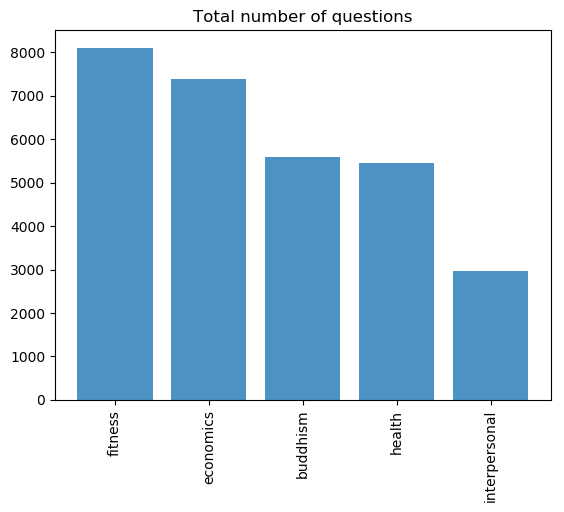
\includegraphics[width=0.5\linewidth]{../../01-python-code/00-workspace/01-graphs/post-counts-bar-graph} \end{center}



\begin{center}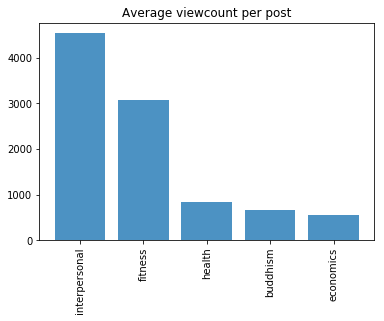
\includegraphics[width=0.5\linewidth]{../../01-python-code/00-workspace/01-graphs/ave-views-bar-graph} \end{center}



\begin{center}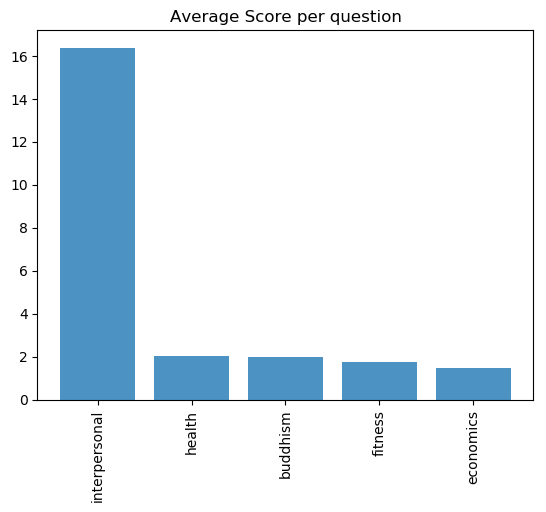
\includegraphics[width=0.5\linewidth]{../../01-python-code/00-workspace/01-graphs/ave-score-bar-graph} \end{center}
\centering
{\footnotesize Source: Own calculations in Python.}
\end{figure}

\normalsize

\begin{figure}
\caption{\textbf{Cumulative Graph for Question Viewcounts}}
\label{fig:cumul}

\begin{center}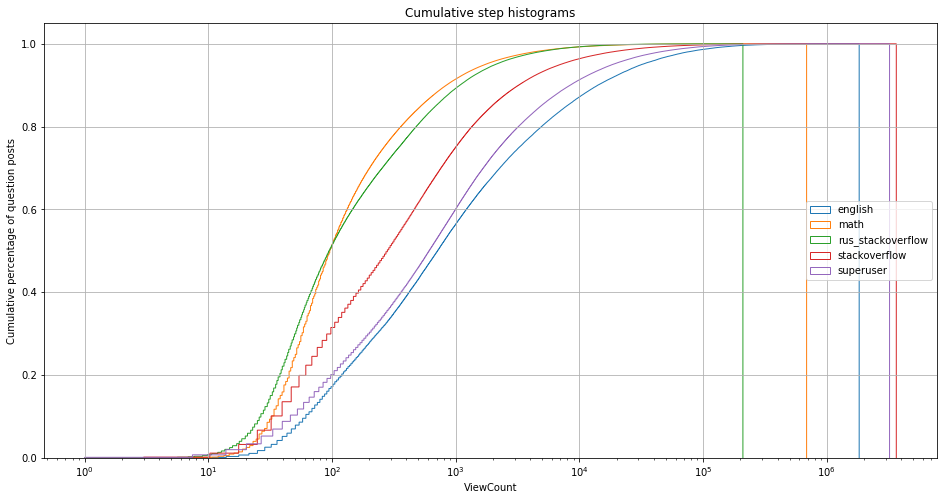
\includegraphics[width=1\linewidth]{../../01-python-code/00-workspace/01-graphs/cumul-viewcount} \end{center}
\centering
{\footnotesize Source: Own calculations in Python.}
\end{figure}

\normalsize

Figure \ref{fig:cumul} plots cumulative percentages of questions as a
function of \texttt{ViewCount} in each fora. There are two aspects of
the graph that are noteworthy - the order of the curves from left to
right, and the fact that they maintain this order (i.e.~they are roughly
parallel). The further right a curve is is indicative of high
\texttt{ViewCounts} per post overall, and we see that this does mirror
the averages calculated in the \texttt{ViewCount} descriptive bar graph
in figure \ref{fig:desc}.

A crossing of curves in figure \ref{fig:cumul} would indicate that there
are certain \texttt{ViewCount} thresholds where a forum becomes more
popular (experiences more viewing traffic) than another. Since there is
very little crossing of curves over all fora, if at all, it appears as
though the distribution of \texttt{ViewCount} across fora is fairly
homogeneous and has relatively constant variance.

\color{black}

\newpage

\section{\texorpdfstring{Methodology
\label{Meth}}{Methodology }}\label{methodology}

\subsection{\texorpdfstring{Empirical Model
\label{Model}}{Empirical Model }}\label{empirical-model}

This is an equation:

\begin{align} \label{eq:EP1}
A_{it}=f(T_i^{(t)},S_i^{(t)},P_i^{(t)},B_i^{(t)},I_i),
\end{align}

\section{\texorpdfstring{Results
\label{Results}}{Results }}\label{results}

\newpage

\section{\texorpdfstring{Recommendations for Further Research
\label{Recom}}{Recommendations for Further Research }}\label{recommendations-for-further-research}

\newpage

\section{\texorpdfstring{Concluding Remarks
\label{Concl}}{Concluding Remarks }}\label{concluding-remarks}

\newpage

\section{References}\label{references}

\hypertarget{refs}{}
\hypertarget{ref-Agichtein2008}{}
Agichtein, E. \emph{et al.} (2008) `Finding high-quality content in
social media', in \emph{Proceedings of the 2008 international conference
on web search and data mining}. ACM, pp. 183--194. doi:
\href{https://doi.org/10.1145/1341531.1341557}{10.1145/1341531.1341557}.

\hypertarget{ref-Berry2017}{}
Berry, G. and Taylor, S. J. (2017) `Discussion quality diffuses in the
digital public square'. Available at:
\url{http://arxiv.org/abs/1702.06677}.

\hypertarget{ref-Bian2009}{}
Bian, J. \emph{et al.} (2009) `Learning to recognize reliable users and
content in social media with coupled mutual reinforcement', in
\emph{Proceedings of the 18th international conference on world wide
web}. ACM, pp. 51--60. doi:
\href{https://doi.org/10.1145/1526709.1526717}{10.1145/1526709.1526717}.

\hypertarget{ref-Gervais2015}{}
Gervais, B. T. (2015) `Incivility Online: Affective and Behavioral
Reactions to Uncivil Political Posts in a Web-based Experiment'. doi:
\href{https://doi.org/10.1080/19331681.2014.997416}{10.1080/19331681.2014.997416}.

\hypertarget{ref-Jeon2006}{}
Jeon, J. \emph{et al.} (2006) `A framework to predict the quality of
answers with non-textual features', in \emph{Proceedings of the 29th
annual international acm sigir conference on research and development in
information retrieval}. ACM, pp. 228--235. doi:
\href{https://doi.org/10.1145/1148170.1148212}{10.1145/1148170.1148212}.

\hypertarget{ref-Li2010}{}
Li, B. and King, I. (2010) `Routing questions to appropriate answerers
in community question answering services', in \emph{Proceedings of the
19th acm international conference on information and knowledge
management}. ACM, pp. 1585--1588. doi:
\href{https://doi.org/10.1145/1871437.1871678}{10.1145/1871437.1871678}.

\hypertarget{ref-Li2012}{}
Li, B. \emph{et al.} (2012) `Analyzing and predicting question quality
in community question answering services', in \emph{Proceedings of the
21st international conference on world wide web}. ACM, pp. 775--782.
doi:
\href{https://doi.org/10.1145/2187980.2188200}{10.1145/2187980.2188200}.

\hypertarget{ref-Li2011}{}
Li, B., King, I. and Lyu, M. R. (2011) `Question routing in community
question answering', in \emph{Proceedings of the 20th acm international
conference on information and knowledge management}. ACM, pp.
2041--2044. doi:
\href{https://doi.org/10.1145/2063576.2063885}{10.1145/2063576.2063885}.

\hypertarget{ref-Liu2008}{}
Liu, Y., Bian, J. and Agichtein, E. (2008) `Predicting information
seeker satisfaction in community question answering', in
\emph{Proceedings of the 31st annual international acm sigir conference
on research and development in information retrieval}. ACM (Section 2),
pp. 483--490. doi:
\href{https://doi.org/10.1145/1390334.1390417}{10.1145/1390334.1390417}.

\hypertarget{ref-Qu2009}{}
Qu, M. \emph{et al.} (2009) `Probabilistic question recommendation for
question answering communities', in \emph{Proceedings of the 18th
international conference on world wide web}. ACM (2), pp. 1229--1230.
doi:
\href{https://doi.org/10.1145/1526709.1526942}{10.1145/1526709.1526942}.

\hypertarget{ref-Ravi2014}{}
Ravi, S. \emph{et al.} (2014) `Great Question! Question Quality in
Community Q\&A.', in \emph{Eighth international aaai conference on
weblogs and social media}. (1), pp. 426--435.

\hypertarget{ref-Riahi2012}{}
Riahi, F. \emph{et al.} (2012) `Finding expert users in community
question answering', in \emph{Proceedings of the 21st international
conference on world wide web}. ACM, pp. 791--798. doi:
\href{https://doi.org/10.1145/2187980.2188202}{10.1145/2187980.2188202}.

\hypertarget{ref-Shah2010}{}
Shah, C. and Pomerantz, J. (2010) `Evaluating and predicting answer
quality in community QA', in \emph{Proceedings of the 33rd international
acm sigir conference on research and development in information
retrieval}. ACM (March 2008), pp. 411--418. doi:
\href{https://doi.org/10.1145/1835449.1835518}{10.1145/1835449.1835518}.

\hypertarget{ref-Shah2018}{}
Shah, V. \emph{et al.} (2018) `Adaptive matching for expert systems with
uncertain task types', in \emph{2017 55th annual allerton conference on
communication, control, and computing (allerton)}. IEEE, pp. 753--760.
doi:
\href{https://doi.org/10.1109/ALLERTON.2017.8262814}{10.1109/ALLERTON.2017.8262814}.

\hypertarget{ref-Sung2013}{}
Sung, J., Lee, J.-g. and Lee, U. (2013) `Booming Up the Long Tails:
Discovering Potentially Contributive Users in Community-Based Question
Answering Services', in \emph{Seventh international aaai conference on
weblogs and social media}, pp. 602--610.

\hypertarget{ref-Szpektor2013}{}
Szpektor, I., Maarek, Y. and Pelleg, D. (2013) `When relevance is not
enough: promoting diversity and freshness in personalized question
recommendation', in \emph{Proceedings of the 22nd international
conference on world wide web}. ACM, pp. 1249--1260.

\hypertarget{ref-Tian2013}{}
Tian, Q., Zhang, P. and Li, B. (2013) `Towards Predicting the Best
Answers in Community-Based Question-Answering Services', in
\emph{Seventh international aaai conference on weblogs and social
media}, pp. 725--728.

\hypertarget{ref-Wu2008}{}
Wu, H., Wang, Y. and Cheng, X. (2008) `Incremental probabilistic latent
semantic analysis for automatic question recommendation', in
\emph{Proceedings of the 2008 acm conference on recommender systems}.
ACM, p. 99. doi:
\href{https://doi.org/10.1145/1454008.1454026}{10.1145/1454008.1454026}.

\hypertarget{ref-Zhou2012}{}
Zhou, T. C., Lyu, M. R. and King, I. (2012) `A classification-based
approach to question routing in community question answering', in
\emph{Proceedings of the 21st international conference on world wide
web}. ACM, pp. 783--790. Available at:
\url{http://www2012.wwwconference.org/proceedings/companion/p783.pdf}.

\newcommand\wordcount{
    \immediate\write18{texcount -sub=section \jobname.tex  | grep "Section" |     sed -e 's/+.*//' | sed -n \thesection p > 'count.txt'}
(\input{count.txt}words)}

\section*{References}

\end{document}
